\chapter{Conclusiones}

\noindent
\lettrine[lines=2, lhang=0.33, loversize=0.25]{\textbf{L}}{as}\
tendencias actuales en cuanto a desarrollo de sofware compuesto\
por inteligencia artificial, se inclinan a favorecer arquitecturas\
que involucran redes neuronales en un rol preponderante. Por ello, esta\
tesis se desarrolló respetando los métodos que indica el \emph{estado del arte}
en cuestión de procesamiento de imágenes y generación de lenguaje natural.\par
El advenimiento de modelos como \emph{Inception V3} en generación de descripciones\
de imágenes fue uno de los precursores más importantes para el crecimiento
del \emph{aprendizaje profundo}. Como consecuencia inmediata, muchos problemas\
de inteligencia artificial pasaron a depender fuertemente de la existencia y extracción\
de grandes cantidades de datos. Por otra parte, es evidente que este proceso es,\
en sí, un área en pleno desarrollo para todo el que se dedique a las \emph{ciencias de datos}%
\footnote{
  Las \emph{ciencias de datos} son un concepto moderno que engloba los métodos interdisciplinarios\
  que involucran estadística, probabilidad, investigación de operaciones y optimización para\
  el procesamiento de grandes cantidades de información.
}. En particular, aquí experimentamos con un conjunto de datos de tamaño pequeño y con\
una estructura distinta a \emph{ImageNet}.\par
El estudio de los memes de Internet es un área poco explorada dentro de aprendizaje profundo.\
A pesar de haber podido reunir un cúmulo de datos clasificados por personaje, en la actualidad\
este orden ya no se sigue. Haciendo una analogía al concepto propuesto por Richard Dawkins,\
el meme es una unidad de información que evoluciona y se transforma: hoy en día la popularidad\
de un meme en una red social se extingue más rápido que hace 4 o 5 años.

\section{El \emph{flujo} de los memes}

\noindent
El problema de la generación de leyendas para memes se trató estrictamente desde un punto\
de vista de aprendizaje automático. Si bien existen algoritmos de optimización que incorporan\
procesos evolutivos de la información, la intención fue explorar la construcción de una\
arquitectura capaz de \emph{extraer características} y procesarlas de manera numérica.\
De ahí que se decidió utilizar modelos convolucionales \emph{``convencionales''} sin conocimiento\
previo al personaje.\par
Vista como tarea de clasificación de imágenes, la extracción de códigos convolucionales resultó\
tener éxito tanto con modelos profundos como superficiales. Entonces, ¿qué tan necesaria es\
una arquitectura de gran profundidad para procesar un conjunto de datos de memes de Internet?\
Para contestar, de manera general a esta pregunta se requiere continuar con la recolección\
y procesamiento de datos, incluyendo los memes que gozan de popularidad hoy en día. Tras los experimentos\
realizados, proponemos que una estructura adecuada involucraría jerarquizar nuevos memes\
en categorías dependiendo de los personajes involucrados.\par
La generación de descripciones para imágenes es una tarea que, en aprendizaje profundo,\
se ha reducido a la optimización de un modelo de lenguaje a partir de representaciones vectoriales\
de un vocabulario. En este contexto, tratamos con un conjunto de textos cortos y con un nivel\
de lenguaje bastante informal: cualquier persona es capaz de etiquetar un personaje de\
\verb+MemeGenerator+ sin importar si el texto hace sentido para los demás \emph{internautas}.\
Por ello es que es complicado analizar si un meme de Internet es correcto, en comparación\
con otros \emph{córpora} en inglés. Teniendo esto en mente, se justifica la existencia de un\
alto porcentaje de leyendas generadas sin sentido pero se destaca la reducción que tuvo la\
perplejidad al evaluar los modelos (Tabla \ref{avgperplexities}) como evidencia de que hubo un\
aprendizaje.\par
El modelo recurrente con unidades LSTM es el \emph{estado del arte} actual en generación de lenguaje\
natural a través de redes neuronales. Debido a que cada personaje posee una personalidad independiente\
a la mayoría, las leyendas de entrenamiento suelen ser distintas para cada uno de éstos. Con el número\
de leyendas por personaje usadas para entrenar los modelos de mejor desempeño (5 y 20), resulta\
totalmente predecible el hecho de no haber podido capturar la ``forma de hablar'' de algún personaje\
en particular. En cambio vemos reflejadas algunas frases cortas que exhiben las maneras con las que\
se lleva a cabo la comunicación a través de Internet. Esto se ve reflejado en resultados como los de\
la Tabla \ref{exp6:anec}.

\section{Trabajo futuro}

\noindent
Todo el seguimiento que se le dio al conjunto de datos de memes fue inspirado en un método de\
aprendizaje supervisado. En este rubro, se proponen algoritmos completamente dependientes de\
grandes cantidades de datos para su desempeño; no obstante, es natural preguntarse a partir\
de qué punto es necesario extraer datos para realizar aprendizaje automático. El entrenamiento\
que se le da a una red neuronal de cierta profundidad permite que ésta sea utilizada posteriormente como\
\emph{sistema experto}, ahorrándose así, el gasto de recursos que implica entrenar una red\
de mayor profundidad.\par
En el problema de agrupación de datos (\emph{clustering}, en inglés) recae gran parte\
de la investigación realizada en aprendizaje no supervisado. En el caso de las imágenes, la confianza\
adquirida en los modelos (profundos) previamente entrenados con conjuntos de datos como \emph{ImageNet}\
nos brindan un método que ya ha sido explorado con satisfacción en trabajos como \cite{DBLP:journals/corr/DundarJC15}.\
Aprovechando la ``correlación'', que en teoría deberían de tener los códigos convolucionales\
de dos imágenes similares, se puede cuantificar la cercanía de ambos mediante métricas de distancia%
\footnote{
  Por ejemplo, distancia euclidiana, similitud coseno o distancia Manhattan
} en un espacio vectorial. La agrupación de memes puede traer como consecuencia una mejora en la elaboración\
de etiquetas, pues previo al entrenamiento de una LSTM, se pueden asociar nuevas características (estados iniciales)
al corpus de entrenamiento.\par
A mediados de 2012, el sitio web \verb+9gag+%
\footnote{
  \url{https://9gag.com}.
} subió considerablemente de popularidad como una plataforma de intercambio \emph{humorístico} a partir de memes.\
Muchos de los personajes engendrados dentro de \verb+MemeGenerator+ evolucionaron y ``cobraron vida''\
en \verb+9gag+. En particular esto se vio reflejado a partir del formato de memes basado en una historieta\
corta, como el de la Figura \ref{9gagmeme}. En este caso, ya no basta con generar una leyenda que describa a\
toda la imagen, pues se trata de una sucesión de eventos. Visto de manera formal, se buscaría modelar\
la interacción entre dos pares $(i_1, s_1)$, $(i_2, s_2)$ provenientes de un conjunto de datos de entrenamiento\
$I \times S$ de imágenes asociadas con leyendas. Una opción interesante para este problema consiste en adaptar\
la arquitectura \emph{Seq2Seq} \cite{DBLP:journals/corr/SutskeverVL14} a la producción de leyendas para cada\
uno de los cuadros de la historieta.

\begin{figure}
  \centering
  
\includegraphics[width=\textwidth]{9gagmeme}
  \caption{
    Un meme tomado de \url{https://9gag.com} que ejemplifica el formato de historietas popularizado
    por dicho sitio web. Algunas variantes de este formato se siguen utilizando en la actualidad.
  }
  \label{9gagmeme}
\end{figure}

\emph{Seq2Seq} es una arquitectura que utiliza dos LSTM's en situaciones donde hay dos modelos de\
lenguaje involucrados (posiblemente distintos uno del otro). Como se observa en la Figura \ref{seq2seq}\
el rol de una LSTM es \textbf{codificar} una secuencia en vectores (parecido a los códigos convolucionales) que\
sirvan de memoria inicial para la otra LSTM que \textbf{decodificará} para producir otra secuencia que siga\
probabilísticamente a la primera mencionada.\par
El éxito de este modelo se ha comprobado principalmente\
en traducción automática de idiomas y, más recientemente, en la elaboración de agentes conversacionales (\emph{chatbots}).
Para incorporar este modelo neuronal en etiquetamiento de historietas de memes, la intuición necesaria\
consiste en considerar un agente racional que está tratando de etiquetar cada uno de los cuadros a partir\
del anterior y de los códigos convolucionales extraídos (como memorias iniciales).

\begin{figure}
  \centering
  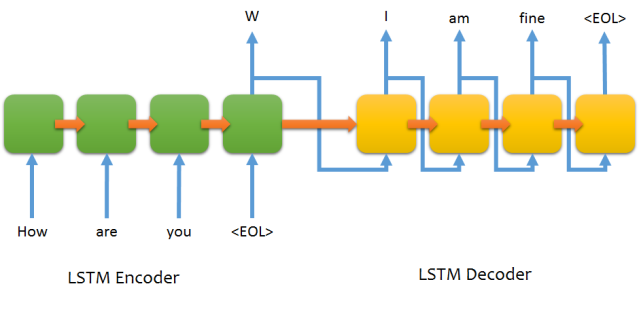
\includegraphics[width=\textwidth]{seq2seq}
  \caption{
    Arquitectura \emph{Seq2Seq} aplicada al aprendizaje de modelos de lenguaje para un agente conversacional.
    Típicamente, se utilizan conjuntos de datos que enseñen al agente a responder preguntas que haría un
    usuario. (Tomado de \url{https://github.com/farizrahman4u/seq2seq.git}).
  }
  \label{seq2seq}
\end{figure}

El meme es la forma de comunicación de la era actual. Richard Dawkins propuso el concepto y los avances\
tecnológicos dieron la plataforma para llevarse a cabo. Así como pueden estudiarse los contenidos de un\
programa de televisión para entender los gustos de la gente, el intercambio de ideas a través de memes\
permite el desarrollo de estrategias que potencialmente influyan en el comportamiento en una gran masa\
de población. Por otro lado, el contenido de la información compactada en un meme significa que detrás\
hay un mecanismo efectivo de compresión de datos que merece ser estudiado tanto en aprendizaje automático\
como en teoría de la información.\par
Si bien es cierto que muchos de los resultados anecdóticos de esta tesis no fueron del todo satisfactorios,\
hay otras maneras de interpretar el conocimiento incrustado en los tensores multidimensionales que produce un\
modelo neuronal. Mediante algoritmos de reducción de dimensiones, combinados con la idea de \emph{clustering}\
presentada anteriormente, la LSTM se vuelve en un método interesante para analizar la semántica con la que\
un agente expuesto al Internet comprende el contenido de una red social.\par
También es importante considerar la volatilidad que existe dentro del \emph{estado del arte} de la inteligencia\
artificial. En la presente década se dieron los medios para el resurgimiento del aprendizaje profundo, pero ello\
no significa que hayamos llegado a la \emph{panacea} algorítmica. Más concretamente, existen fuertes críticas\
hacia las redes convolucionales, las cuales han ido creciendo a pesar de que aún no se tenga un modelo que las supere.\
Geoffrey Hinton, uno de los \emph{padres} del aprendizaje profundo, ha sido uno de los entusiastas\
de este movimiento, sobre todo al publicar un nuevo modelo neuronal para el procesamiento de imágenes \cite{2017arXiv171009829S}.\
Inmediatamente surge la inquietud de si este nuevo modelo puede mejorar el desempeño expuesto en esta tesis y\
para un conjunto de datos semejante al de memes con el que se trabajó.\par
Para finalizar, vale la pena recordar el famoso ``teorema'' del \textbf{no almuerzo gratis} (\emph{no-free lunch theorem})\
que tanto caracteriza al aprendizaje automático hoy en día: si un modelo $M$ tuvo éxito para una tarea $X$, no significa\
que éste va a dar respuesta a otra tarea $Y$. Hasta ahora, el \emph{boom} del aprendizaje profundo ha traído\
grandes avances en inteligencia artificial especializada por tareas particulares. Si buscamos extender la comprensión\
de entes de información, como memes, caemos dentro de la inteligencia artificial general, un campo de estudio\
muchas veces teórico el cual prioriza el entendimiento y la construcción de máquinas similares al ser humano.\
¿Vale la pena estudiar memes? ¿Qué sería de nuestra existencia en el siglo $XXI$ si no fuera por las mentes más\
curiosas del siglo $XX$?\par
\begin{center}
  \emph{``Ars longa, vita brevis.''}
  \\[5pt]
  --- Hipócrates
\end{center}

\newpage
